% Fig: worked example, benchmark S2 in SSA form and after optimization.
% Block contents are copied from the pipeline's output (paper_eval/pipeline.py).
\documentclass[border=2pt]{standalone}
\usepackage{mathptmx}
\usepackage{tikz}
\usetikzlibrary{arrows.meta,positioning,fit,backgrounds}
\newcommand{\phin}{\textbf{phi}}
\begin{document}
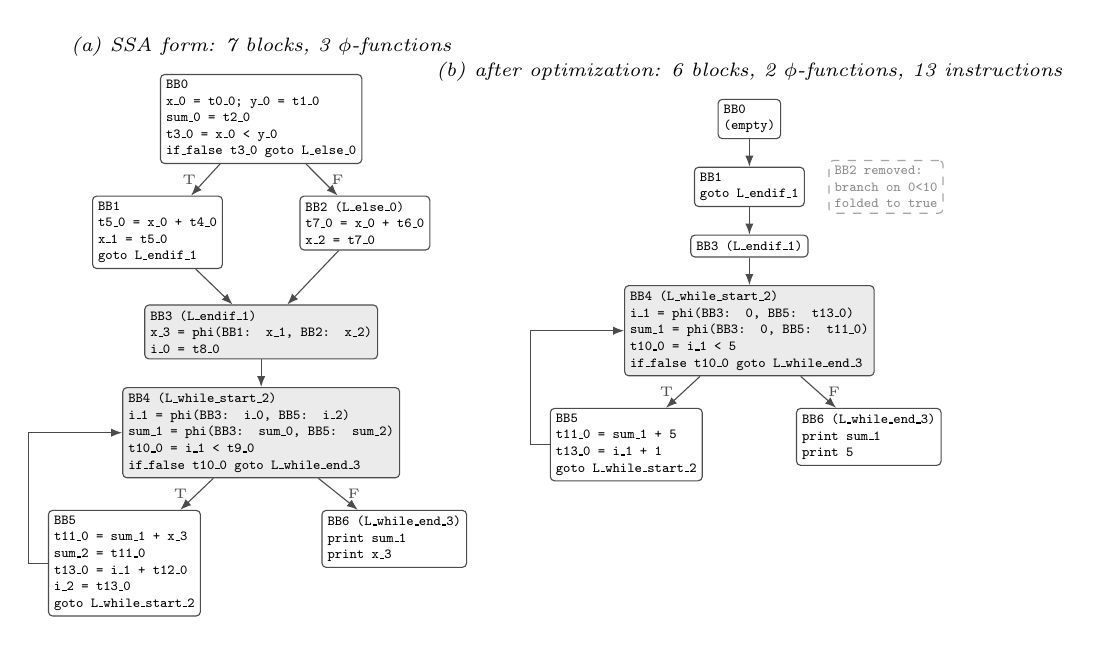
\begin{tikzpicture}[
  font=\tiny,
  bb/.style={draw=black!70, rounded corners=1.5pt, fill=white, align=left, inner sep=2pt, font=\tiny\ttfamily},
  phi/.style={bb, fill=black!8},
  arr/.style={-{Latex[length=1.4mm]}, black!70},
  dead/.style={bb, draw=black!35, text=black!45, dashed},
  lbl/.style={font=\scriptsize\itshape}]
  % ---------------- (a) SSA form
  \node[bb] (b0) at (0,0) {BB0\\ x\_0 = t0\_0;\ y\_0 = t1\_0\\ sum\_0 = t2\_0\\ t3\_0 = x\_0 < y\_0\\ if\_false t3\_0 goto L\_else\_0};
  \node[bb, below left=4mm and -8mm of b0] (b1) {BB1\\ t5\_0 = x\_0 + t4\_0\\ x\_1 = t5\_0\\ goto L\_endif\_1};
  \node[bb, below right=4mm and -8mm of b0] (b2) {BB2 (L\_else\_0)\\ t7\_0 = x\_0 + t6\_0\\ x\_2 = t7\_0};
  \node[phi, anchor=north] (b3) at ([yshift=-4.5mm] b0.south |- b1.south) {BB3 (L\_endif\_1)\\ x\_3 = \phin(BB1: x\_1, BB2: x\_2)\\ i\_0 = t8\_0};
  \node[phi, below=3.5mm of b3] (b4) {BB4 (L\_while\_start\_2)\\ i\_1 = \phin(BB3: i\_0, BB5: i\_2)\\ sum\_1 = \phin(BB3: sum\_0, BB5: sum\_2)\\ t10\_0 = i\_1 < t9\_0\\ if\_false t10\_0 goto L\_while\_end\_3};
  \node[bb, below left=4mm and -10mm of b4] (b5) {BB5\\ t11\_0 = sum\_1 + x\_3\\ sum\_2 = t11\_0\\ t13\_0 = i\_1 + t12\_0\\ i\_2 = t13\_0\\ goto L\_while\_start\_2};
  \node[bb, below right=4mm and -10mm of b4] (b6) {BB6 (L\_while\_end\_3)\\ print sum\_1\\ print x\_3};
  \draw[arr] (b0) -- node[left, font=\tiny]{T} (b1);
  \draw[arr] (b0) -- node[right, font=\tiny]{F} (b2);
  \draw[arr] (b1) -- (b3);
  \draw[arr] (b2) -- (b3);
  \draw[arr] (b3) -- (b4);
  \draw[arr] (b4) -- node[left, font=\tiny]{T} (b5);
  \draw[arr] (b4) -- node[right, font=\tiny]{F} (b6);
  \draw[arr] (b5.west) -- ++(-2.5mm,0) |- (b4.west);
  \node[lbl, above=1mm of b0] {(a) SSA form: 7 blocks, 3 $\phi$-functions};
  % ---------------- (b) optimized
  \begin{scope}[xshift=62mm]
  \node[bb] (o0) at (0,0) {BB0\\ (empty)};
  \node[bb, below=3.5mm of o0] (o1) {BB1\\ goto L\_endif\_1};
  \node[dead, right=3mm of o1] (o2) {BB2 removed:\\ branch on 0<10\\ folded to true};
  \node[bb, below=3.5mm of o1] (o3) {BB3 (L\_endif\_1)};
  \node[phi, below=3.5mm of o3] (o4) {BB4 (L\_while\_start\_2)\\ i\_1 = \phin(BB3: 0, BB5: t13\_0)\\ sum\_1 = \phin(BB3: 0, BB5: t11\_0)\\ t10\_0 = i\_1 < 5\\ if\_false t10\_0 goto L\_while\_end\_3};
  \node[bb, below left=4mm and -10mm of o4] (o5) {BB5\\ t11\_0 = sum\_1 + 5\\ t13\_0 = i\_1 + 1\\ goto L\_while\_start\_2};
  \node[bb, below right=4mm and -10mm of o4] (o6) {BB6 (L\_while\_end\_3)\\ print sum\_1\\ print 5};
  \draw[arr] (o0) -- (o1);
  \draw[arr] (o1) -- (o3);
  \draw[arr] (o3) -- (o4);
  \draw[arr] (o4) -- node[left, font=\tiny]{T} (o5);
  \draw[arr] (o4) -- node[right, font=\tiny]{F} (o6);
  \draw[arr] (o5.west) -- ++(-2.5mm,0) |- (o4.west);
  \node[lbl, above=1mm of o0] {(b) after optimization: 6 blocks, 2 $\phi$-functions, 13 instructions};
  \end{scope}
\end{tikzpicture}
\end{document}
